\documentclass{beamer}
\usepackage{ragged2e}
\usepackage{CJKutf8}
\usepackage{tikz}
\setbeamertemplate{theorems}[numbered]
\justifying\let\raggedright\justifying
\begin{document}
\begin{CJK*}{UTF8}{gbsn}

\newtheorem{Thm}{定理}[section]
\theoremstyle{definition}
\newtheorem{Def}{定义}[section]
\theoremstyle{example}
\newtheorem*{Ex}{例:}
\newtheorem{Exercise}{习题}

\date{}
\author{陈建文}

\title{逻辑初步}
\begin{frame}
  \titlepage
\end{frame}  
\section{课程学习目标}
\begin{frame}
  \frametitle{请同学们加入课程QQ群,QQ群号:740716920}
  修改群昵称为"123456789姓名"的样式,
  
  其中"123456789"为自己的学号。

  \includegraphics[]{qq.png}
\end{frame}
\begin{frame}
  \frametitle{课程成绩要求}

  课程总成绩=MOOC成绩+平时作业成绩+期末考试成绩

其中:

MOOC成绩:20\%

(MOOC《集合论与图论(上)》总成绩+MOOC《集合论与图论(下)》总成绩)/2 * 20\%


平时作业成绩:10\%


期末考试:70\%


教务处课表规定的教室上课时间每缺勤一次从总成绩中扣2分!只有期末考试卷面成绩达到90分以上者可以免除缺勤扣分。
\end{frame}
\begin{frame}
  \frametitle{课程学习目标}
\begin{enumerate}
\item 提升逻辑思维能力
\item 提升抽象思维能力
\item 提升利用数学语言准确描述计算机科学问题和电子信息科学问题的能力
\end{enumerate}

\end{frame}
\begin{frame}
  "如果不理解它的语言,没有人能读懂宇宙这本伟大的书,它的语言就是数学"
  --伽利略(1564-1642)
\end{frame}
\begin{frame}
    命题:可以判断真假的陈述句。通常,我们用$T$表示真,用$F$表示假。
  \begin{Ex}\quad   
    \begin{enumerate}
    \item 对任意的自然数$a,b,c$,$(a + b) + c = a + (b + c)$。(真命题)
    \item $\sqrt{2}$是无理数。(真命题)
    \item $\sqrt{2}$是有理数。(假命题)
    \item 设$f:[a,b] \to R$为一个Riemann可积函数,$F:[a,b] \to R$在$[a,b]$上满足$F'(x)=f(x)$,那么$\int_{a}^{b}f(x)dx = F(b) - F(a)$。(真命题)
    \item 任何一幅地图都可以用四种颜色进行着色,使得相邻的区域着以不同的颜色。
    \end{enumerate}
  \end{Ex}
\end{frame}

\begin{frame}
  \centering
  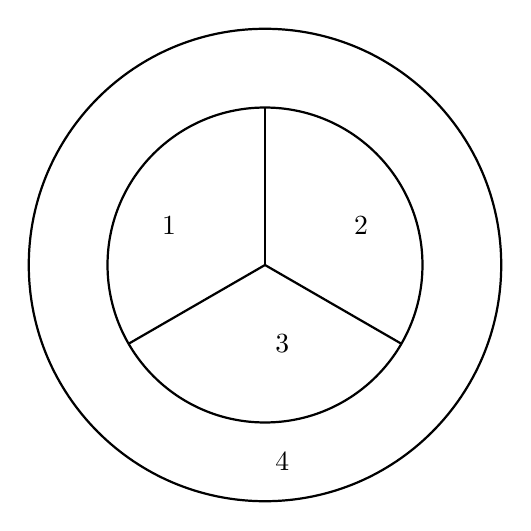
\begin{tikzpicture}[thick]
    \draw (0,0) circle [radius=2cm];
    \draw (0,0) circle [radius=3cm];
    \draw (0,0) -- (0,2);
    \draw (0,0) -- (-1.732, -1.0);
    \draw (0,0) -- (1.732, -1.0);
    \draw (-1,0.5) node[left] {$1$};
    \draw (1,0.5) node[right] {$2$};
    \draw (0,-1) node[right] {$3$};
    \draw (0,-2.5) node[right] {$4$};
  \end{tikzpicture}

\end{frame}

\begin{frame}
    谓词:命题的谓语部分。
  
  \begin{Ex}\quad
    
    \begin{description}
    \item     [$P(x): x$ 是偶数] 这里$P$为一元谓词,表示“是偶数”。当$x$为某个确定的数字时,$P(x)$则对应一个命题。例如$P(2)$为真命题,$P(1)$为假命题。这里,$P$之所以被称为一元谓词,是因为$P(x)$只包含一个变量$x$。
    \item     [$P(x,y): x >y$]  这里$P$为二元谓词,表示$>$。当$x$和$y$为确定的数字时,$P(x,y)$则对应一个命题。例如$1>0$为真命题,$0>1$为假命题。这里,$P$之所以被称为二元谓词,是因为$P(x,y)$包含两个变量$x$和$y$。
    \end{description}
相应的,有三元谓词,四元谓词,......
\end{Ex}
\end{frame}
\begin{frame}
  我们还可以用如下方式由谓词得到命题:

\begin{description}
\item [$\forall x P(x)$:] 对任意的$x$,$P(x)$。For All中的$A$上下颠倒可以得到$\forall$。
\item [$\exists x P(x)$:] 存在$x$,$P(x)$。There Exists中的$E$左右颠倒可以得到$\exists$。
\end{description}

\end{frame}
\begin{frame}
  \frametitle{复合命题}
  设$p$为命题,则$\lnot p$表示“$p$不成立”。

 \begin{tabular}{c|c}
    p& $\lnot$ p\\
    \hline
    T&F\\
    F&T\\
  \end{tabular}

\end{frame}
\begin{frame}
    \frametitle{复合命题}
    设$p$和$q$为两个命题,则$p\land q$表示“$p$成立,并且$q$成立”。
  
  \begin{tabular}{cc|c}
    p& q& p $\land$ q\\
    \hline
    T&T&T\\
    T&F&F\\
    F&T&F\\
    F&F&F\\
  \end{tabular}

\end{frame}
\begin{frame}
    \frametitle{复合命题}

    设$p$和$q$为两个命题,则$p\lor q$表示“$p$成立,或者$q$成立”。
  
  \begin{tabular}{cc|c}
    p& q& p $\lor$ q\\
    \hline
    T&T&T\\
    T&F&T\\
    F&T&T\\
    F&F&F\\
  \end{tabular}

\end{frame}
\begin{frame}
    \frametitle{复合命题}
  设$p$和$q$为两个命题,则$p\to q$表示“如果$p$成立,那么$q$成立”。  

    \begin{tabular}{cc|c}
    p& q& p $\to$ q\\
    \hline
    T&T&T\\
    T&F&F\\
    F&T&T\\
    F&F&T\\
    \end{tabular}
    \begin{minipage}{0.8\linewidth}
      \pause
      $\forall x \; x > 1 \to x^2 > 1$

      \pause
      1)当$x=2$时, $2 > 1 \to 2^2 >1$成立,这对应于真值表的第一行;

      \pause
    2)当$x=0$时,$0 > 1 \to 0^2 > 1$成立,这对应于真值表的第四行;

      \pause
    3)当$x=-2$时,$-2>1 \to (-2)^2 > 1$成立,这对应于真值表的第三行。
    \end{minipage}
   
  \end{frame}
  \begin{frame}
      \frametitle{复合命题}
    设$p$和$q$为两个命题,则$p\leftrightarrow q$表示“$p$等价于$q$”。  

  \begin{tabular}{cc|c}
    p& q& p $\leftrightarrow$ q\\
    \hline
    T&T&T\\
    T&F&F\\
    F&T&F\\
    F&F&T\\
  \end{tabular}
\end{frame}
\begin{frame}
\frametitle{$p\land (q\lor r)$与$(p\land q)\lor (p \land r)$是等价的。}
\begin{tabular}{ccc|cc}
  $p$& $q$& $r$& $p\land (q\lor r)$&$(p\land q)\lor (p \land r)$\\
  \hline
 T& T&T&T&T\\
  T&T&F&T&T\\
  T&F&T&T&T\\
   T& F&F&F&F\\
  F&T&T&F&F\\
  F&T&F&F&F\\
 F& F&T&F&F\\
  F&  F&F&F&F\\      
\end{tabular}
\end{frame}
\begin{frame}
  \frametitle{$p\lor (q\land r)$与$(p\lor q)\land (p \lor r)$是等价的。}
  \begin{tabular}{ccc|cc}
    $p$& $q$& $r$&$p\lor (q\land r)$ &$(p\lor q)\land (p \lor r)$\\
    \hline
    T&T&T&T&T\\
    T&T&F&T&T\\
    T&F&T&T&T\\
     T& F&F&T&T\\
    F&T&T&T&T\\
    F&T&F&F&F\\
    F&F&T&F&F\\
     F&F&F&F&F\\
  \end{tabular}
\end{frame}
\begin{frame}
  \frametitle{$\lnot (p\land q)$与$\lnot p \lor \lnot q$是等价的。}
  \begin{tabular}{cc|cc}
    $p$& $q$&$\lnot (p\land q)$ &$\lnot p \lor \lnot q$\\
    \hline
    T&T&F&F\\
    T&F&T&T\\
    F&T&T&T\\
      F&F&T&T\\      
  \end{tabular}
\end{frame}
\begin{frame}
  \frametitle{$\lnot (p \lor q)$与$\lnot p \land \lnot q$是等价的。}
  \begin{tabular}{cc|cc}
    $p$& $q$&$\lnot (p \lor q)$&$\lnot p \land \lnot q$\\
    \hline
    T&T&F&F\\
    T&F&F&F\\
    F&T&F&F\\
    F&F&T&T\\      
  \end{tabular}
\end{frame}

\begin{frame}
  \frametitle{$p \to q$与$\lnot p \lor q$是等价的。}
  \begin{tabular}{cc|cc}
    $p$& $q$&$p \to q$&$\lnot p \lor q$\\
    \hline
    T&T&T&T\\
    T&F&F&F\\
    F&T&T&T\\
    F&F&T&T\\      
  \end{tabular}
  
\end{frame}

\begin{frame}
  “如果$p$成立,那么$q$成立。”这句话的否定是()

  A. “如果$p$成立,那么$q$不成立。”

  B. “$p$成立并且$q$不成立。”

\pause
  \begin{equation*}
    \begin{split}
  & \lnot (p \to q)\\
  \Leftrightarrow & \lnot (\lnot p \lor q)\\
   \Leftrightarrow & \lnot (\lnot p) \land \lnot q\\
    \Leftrightarrow & p \land \lnot q
    \end{split}
  \end{equation*}
\end{frame}

\begin{frame}
    \frametitle{一些逻辑术语的约定}
    The negation of a proposition $P$: $\lnot P$

  命题$P$的否定:$\lnot P$

  The converse of $P\to Q$: $Q \to P$

  命题$P\to Q$的逆命题:$Q\to P$



  The inverse of $P\to Q$: $\lnot P \to \lnot Q$
  
  在较深入的探讨数理逻辑的教材中,该概念用的很少,因此我们不给出具体的翻译称谓,在需要表达该概念时明确说明为$\lnot P \to \lnot Q$即可。

  
  The contrapositive of $P\to Q$: $\lnot Q \to \lnot P$

  命题$P\to Q$的逆否命题:$\lnot Q \to \lnot P$

  需要特别说明的是,命题$P\to Q$的否定为$\lnot (P \to Q)$,而不是$P \to \lnot Q$。 
\end{frame}
\end{CJK*}
\end{document}
